\begin{comment}
\addbibresource{referencias/Referencias.bib}
\end{comment}

\section{Marco Teórico}
\label{sc:teoria}

\subsection{Ecuación Constitutiva}
Las bases de la teoría no local las sentó \textcite{Kroner1967} en su artículo \textit{\citetitle*{Kroner1967}}. En este, Kröner expone que la energía sobre un cristal cúbico primitivo se debe en parte a las fuerzas de corto alcance y en parte a las fuerzas de largo alcance, de tal manera, Kröner llega a la siguiente ecuación:
\begin{equation}
	E=\frac{1}{2}\left[\int_{V}C_{ijkl}\varepsilon_{ij}(\boldsymbol{x})\varepsilon_{kl}(\boldsymbol{x})dv\right]+\frac{1}{2}\left[\int_{V}\int_{V'}C_{ijkl}(\boldsymbol{x})\varepsilon_{ij}(\boldsymbol{x})\varepsilon_{kl}(\boldsymbol{x'})dv'dv\right]
\end{equation}
Por ello, Kröner adopta el término No local para referirse a la interacción de fuerzas de largo alcance que se representan en el segundo término de la parte derecha de la ecuación.

Con ello, Kröner llegó a la siguiente ecuación constitutiva:
\begin{equation}
	\sigma_{ij}(\boldsymbol{x})=C_{ijkl}\varepsilon_{kl}(\boldsymbol{x})+\int_{v'}C_{ijkl}(|\boldsymbol{x}-\boldsymbol{x'}|)\varepsilon_{kl}(\boldsymbol{x})dv'
\end{equation}
En esta ecuación, el segundo término representa el aporte no local mientras que el primer término representa el aporte local clásico. Además, se introduce el tensor $C_{ijkl}(|\boldsymbol{x}-\boldsymbol{x'}|)$ llamado el tensor elástico material. Este tensor depende de la distancia entre el punto de interés y los puntos del dominio. En este punto, no existía una manera sencilla de calcular $C_{ijkl}(|\boldsymbol{x}-\boldsymbol{x'}|)$.

No fue hasta 5 años después que \textcite{Eringen1972} desarrollaron un modelo matemático donde se formula de manera completa la elasticidad no local. De este trabajo nace la teoría lineal en la que \textcite{Eringen1987} describe los dos modelos de elasticidad no local y sus aplicaciones. Los dos modelos son el modelo integral, el cual describe la interacción de fuerzas a larga distancia, y el modelo diferencial que describe interacciones a corta distancia \parencite{Polizzotto2001}. Eringen muestra una gran variedad de problemas que se pueden solucionar con la teoría no local, entre los que destacan la propagación de ondas y el uso de esta teoría en el estudio de fractura y grietas. Esto se debe a que en las puntas de las grietas, la elasticidad local presenta singularidades, obteniendo así un esfuerzo infinito, mientras que en la teoría no local hay un aporte del volumen adyacente, lo cual evita tener esfuerzos infinitos \parencite{Eringen1987}. 

En el trabajo \citetitle*{Eringen1987}, Eringen expone una manera de calcular el tensor elástico material.
\begin{equation}
	C_{ijkl}(|\boldsymbol{x}-\boldsymbol{x'}|)=\alpha(|\boldsymbol{x}-\boldsymbol{x'}|)C_{ijkl}
\end{equation}
Donde se introduce $\alpha$ como la \textit{función de atenuación} (este nombre será modificado posteriormente), por lo que Eringen llega a la siguiente ecuación constitutiva:
\begin{equation}
	\sigma_{ij}(\boldsymbol{x})=\int_{v'}\alpha(|\boldsymbol{x}-\boldsymbol{x'}|)C_{ijkl}\varepsilon_{kl}(\boldsymbol{x'})dv'
	\label{eq:eringen}
\end{equation}
A partir de aquí, se resaltan los trabajos de \textcite{Polizzotto2001} donde reporta que la ecuación constitutiva se escribe con un factor $\zeta_1$ y $\zeta_2$, donde $\zeta_1+\zeta_2=1$ con el objetivo de representar el proceso de deformación de un sólido con dos fases. Una fase local ($\zeta_1$) y una fase no local ($\zeta_2$).
\begin{equation}
	\sigma_{ij}(\boldsymbol{x})=\zeta_1C_{ijkl}\varepsilon_{kl}(\boldsymbol{x})+\zeta_2\int_{v'}A(|\boldsymbol{x}-\boldsymbol{x'}|)C_{ijkl}\varepsilon_{kl}(\boldsymbol{x'})dv'
	\label{eq:polizzotto}
\end{equation}
Donde $A$ también es llamada función de atenuación pero $A\neq\alpha$.
Para efectos de este estudio se llamará a la función $\alpha$ como función de difusión y se llamará a la función $A$ función de atenuación.

Por último, en la ecuación \ref{eq:eringen} se tiene dos parámetros locales (Modulo de Young y coeficiente de Poisson) y un parámetro no local (longitud interna $l$), sin embargo, en la ecuación \ref{eq:polizzotto} se cuenta con el parámetro adicional $\zeta_1$.
\subsection{Funciones de Atenuación y Difusión}

Las funciones de difusión que expone \textcite{Eringen1987} deben cumplir con unos requerimientos mínimos que son:
\begin{equation}
	\lim_{l\to0}\alpha=1
\end{equation}
\begin{equation}
	\alpha(0)=1
\end{equation}
Adicionalmente, para que exista una única solución, $\alpha>0$ \parencite{ALTAN19891271}.

Las funciones de atenuación que expone \textcite{Polizzotto2001} deben cumplir con unos requerimientos mínimos que son:

\begin{enumerate}
	\item[] \begin{equation}\lim_{l\to0}A=0\end{equation}
	\item[] \begin{equation}\int_{v^{\infty}}A(|\boldsymbol{x}-\boldsymbol{x'}|)dv'=1
	\label{eq:condicion}
	\end{equation}
\end{enumerate}

A partir de las ecuaciones \ref{eq:eringen},\ref{eq:polizzotto} \textcite{Polizzotto2001} establece la siguiente relación:
\begin{equation}
	\alpha(\rho)=\zeta_1A(\rho)+\zeta_1\delta_{x-x'}
\end{equation}
Donde $\rho=\frac{r}{l}$ y $r=|\boldsymbol{x}-\boldsymbol{x'}|$. $r$ es interpretado comúnmente como la distancia euclidiana.

Como lo enuncia \textcite{ALTAN19891271}, $A$ no tiene que ser necesariamente positiva, por lo que se puede elegir de una gran gama de funciones. En este estudio se analizarán 4 funciones de atenuación y su influencia en los resultados obtenidos variando sus parámetros no locales. Las funciones de atenuación son de la forma:
\begin{equation}
	A(\rho)=\lambda_0f(\rho)
\end{equation}
Donde $\lambda_0$ es un factor de corrección para obligar a cumplir con la condición de $\int_{v^{\infty}}A(|\boldsymbol{x}-\boldsymbol{x'}|)dv'=1$

En la literatura se exponen varias funciones de atenuación de las que resaltan:

Nota: el paréntesis $<f(x)>$ representa el operador de Macauley.
\begin{enumerate}
	\item Función Biexponencial (Función 1)

	\begin{equation}
		A(\rho)=\lambda_0e^{-\rho}
	\end{equation}
	\begin{figure}
	    \centering
	    \sffamily
	    \begin{subfigure}{0.45\textwidth}
	    \centering
	        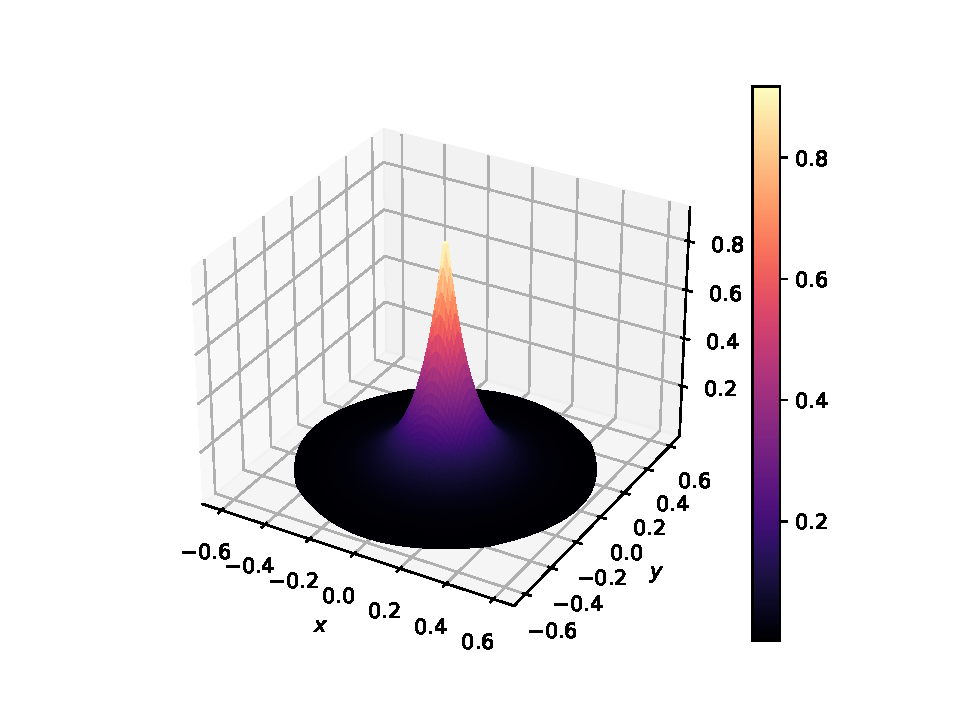
\includegraphics[width=\textwidth]{figuras/biexp3d.pdf}
	        \caption{Superficie tridimensional}
	        \label{fig:biexponencial.3d}
	    \end{subfigure}
	    \begin{subfigure}{0.45\textwidth}
	    \centering
	        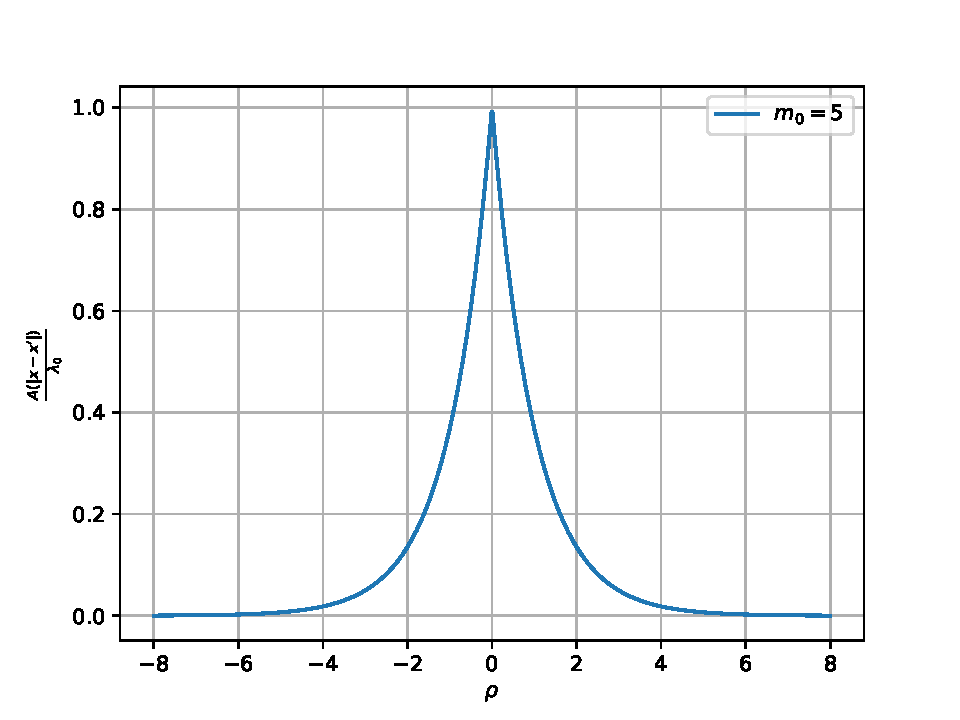
\includegraphics[width=\textwidth]{figuras/biexp2d.pdf}
	        \caption{Corte transversal}
	        \label{fig:biexponencial.2d}
	    \end{subfigure}
	    \caption{Función biexponencial centrada en 0,0}
	    \label{fig:biexponencial}
	\end{figure}

	\item Función Cónica (Función 2)
	\begin{equation}
		A(\rho)=\lambda_0\left<1-\frac{\rho}{(1+m_0)}\right>
	\end{equation}
	\begin{figure}
	    \centering
	    \sffamily
	    \begin{subfigure}{0.45\textwidth}
	    \centering
	        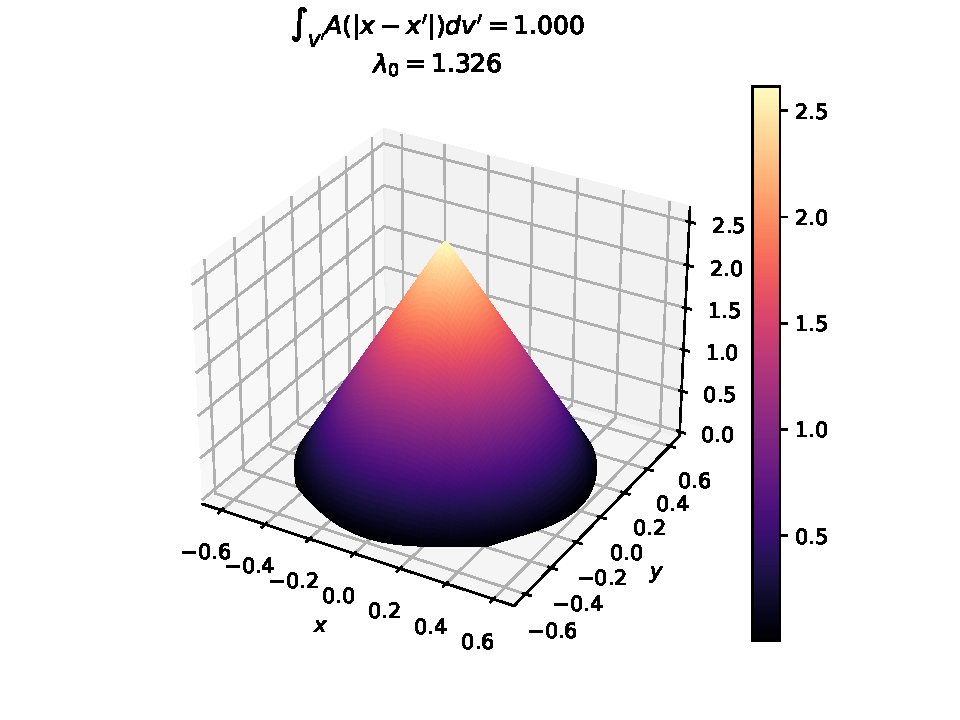
\includegraphics[width=\textwidth]{figuras/conica3d.pdf}
	        \caption{Superficie tridimensional}
	        \label{fig:conica.3d}
	    \end{subfigure}
	    \begin{subfigure}{0.45\textwidth}
	    \centering
	        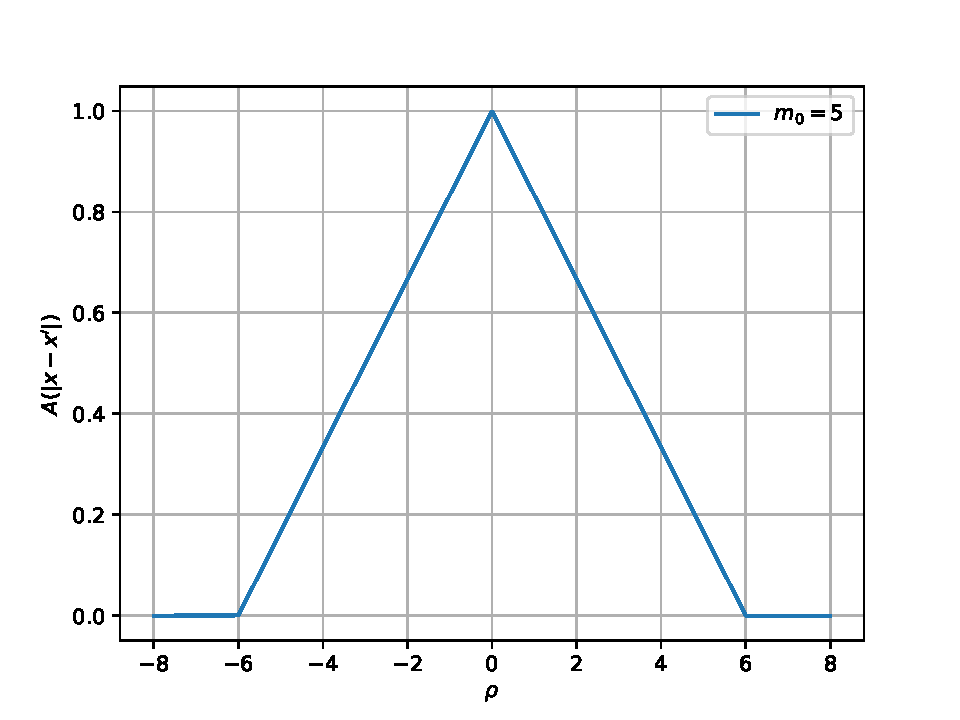
\includegraphics[width=\textwidth]{figuras/conica2d.pdf}
	        \caption{Corte transversal}
	        \label{fig:conica.2d}
	    \end{subfigure}
	    \caption{Función cónica centrada en 0,0}
	    \label{fig:conica}
	\end{figure}

	\item Función Campana (Función 3)
	\begin{equation}
		A(\rho)=\lambda_0\left<1-\frac{\rho^2}{(1+m_0)^2}\right>
	\end{equation}
	\begin{figure}
	    \centering
	    \sffamily
	    \begin{subfigure}{0.45\textwidth}
	    \centering
	        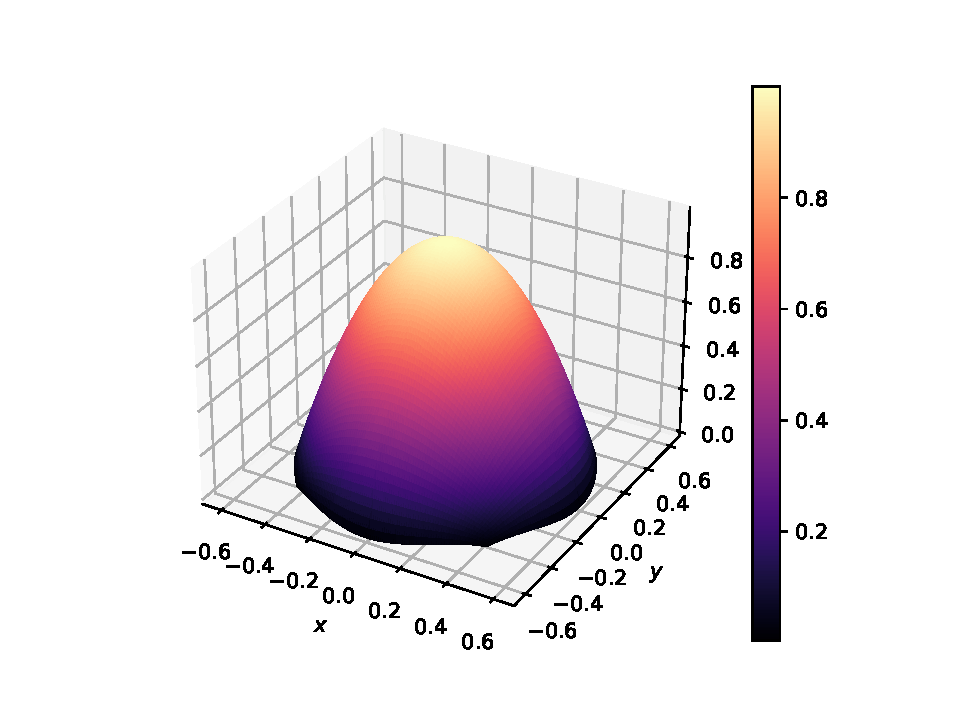
\includegraphics[width=\textwidth]{figuras/campana3d.pdf}
	        \caption{Superficie tridimensional}
	        \label{fig:campana.3d}
	    \end{subfigure}
	    \begin{subfigure}{0.45\textwidth}
	    \centering
	        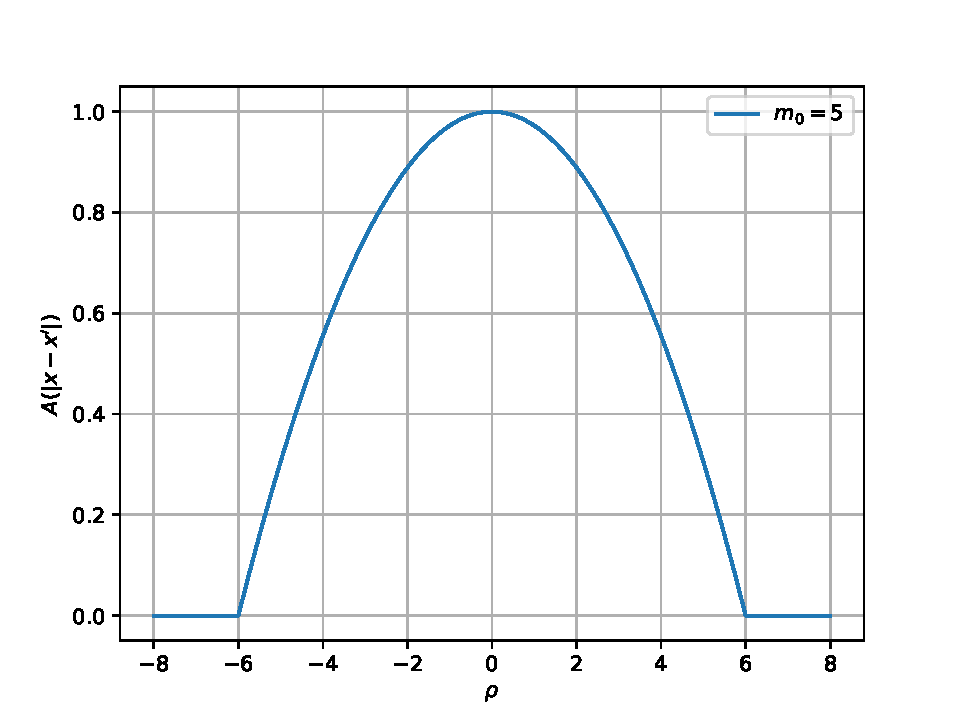
\includegraphics[width=\textwidth]{figuras/campana2d.pdf}
	        \caption{Corte transversal}
	        \label{fig:campana.2d}
	    \end{subfigure}
	    \caption{Función campana centrada en 0,0}
	    \label{fig:campana}
	\end{figure}
\end{enumerate}

Cada una de estas funciones tiene un identificador (Función i) que será usado posteriormente en el desarrollo de los programas.
\subsection{Distancia de influencia \texorpdfstring{$Lr$}{Lr}}

Si se observa el comportamiento de la figura \ref{fig:biexponencial.2d}, se puede apreciar que el valor de la función de atenuación es muy cercana a 0 cuando $|\rho|>=6$. Es por eso que \textcite{Polizzotto2001} define que los efectos no locales solamente se deben tener en cuenta a una distancia máxima $Lr=6l$. Esta afirmación hace que al momento de enmallar un dominio de elementos finitos deba tenerse en cuenta una propiedad material ($l$) para poder modelar el problema no local de manera correcta. Para efectos de este estudio se tomará $Lr=6l$. 

\textcite{Polizzotto2001} propone un parámetro $m_0\geq1$ donde $Lr=(1+m_0)l$. En las figuras \ref{fig:biexponencial.2d} y \ref{fig:biexponencial.2d} se usa dicho parámetro. El parámetro obliga a que $A(\rho)=0$ cuando $|\rho|>(1+m_0)$. Este comportamiento hace que las funciones de atenuación sean comparables entre sí.

\subsection{Factor de corrección \texorpdfstring{$\lambda_0$}{λ0}}

Una vez definidas las funciones de atenuación, basta con hallar el factor $\lambda_0$ para que se cumpla la condición de la ecuación \ref{eq:condicion}.

Dado que $\lambda_0$ es constante, el proceso para encontrar dicho valor se simplifica. De tal manera, se encuentra el valor de la integral en un dominio circular infinito. Se toma como punto base el origen, ya que, el valor de la integral no depende de la posición base sino de los puntos adyacentes a esta base.

\begin{equation}
	t\int_{0}^{2\pi}\int_{0}^{\infty}{rA(r/l)}{dr}{d\theta}=1
\end{equation} 
Donde $r$ es la distancia euclidiana al origen, que en coordenadas polares puede escribirse como el radio.

Note que esta integral se define como integral de área, sin embargo, la integral de la ecuación \ref{eq:condicion} es una integral volumétrica. Se asume un grosor constante por lo que basta con multiplicar por t.

Usando la función 1 como referencia se tiene:

\begin{equation}
	t\lambda_0\int_{0}^{2\pi}\int_{0}^{\infty}{re^{-r/l}}{dr}{d\theta}=1
\end{equation} 

\begin{equation}
	2\pi\lambda_0t\int_{0}^{\infty}{re^{-r/l}}{dr}=1
\end{equation}
\begin{equation}
	2\pi\lambda_0t\int_{0}^{\infty}{re^{-r/l}}{dr}=1
\end{equation} 
\begin{equation}
	2\pi\lambda_0t\left(\lim_{r\to\infty}-e^{\frac{-r}{l}}l^2-lre^{\frac{-r}{l}}+l^2\right)=1
\end{equation} 
\begin{equation}
	2\pi\lambda_0l^2t=1
\end{equation} 

Solucionando para $\lambda_0$:
\begin{equation}
	\lambda_0=\frac{1}{2\pi l^2 t}
\end{equation} 

Para las funciones 2 y 3 se debe modificar el proceso así:
\begin{equation}
	t\int_{0}^{2\pi}\int_{0}^{\infty}{rA(r/l)}{dr}{d\theta}=t\int_{0}^{2\pi}\int_{0}^{Lr}{rA(r/l)}{dr}{d\theta}+t\int_{0}^{2\pi}\int_{Lr}^{\infty}{rA(r/l)}{dr}{d\theta}
\end{equation}
Debido a la definición de la función 2 y 3 es evidente que:
\begin{equation}
	t\int_{0}^{2\pi}\int_{Lr}^{\infty}{rA(r/l)}{dr}{d\theta}=0
\end{equation}

Por lo que el proceso para la función 2 y 3 se simplifica a:
\begin{equation}
	t\int_{0}^{2\pi}\int_{0}^{Lr}{rA(r/l)}{dr}{d\theta}=1
\end{equation}
Al realizar esta simplificación las funciones de atenuación pierden la propiedad del operador de Macauley, ya que, en este intervalo son positivas.

Resolviendo para ambos casos se obtuvo:

Para la función 2:
\begin{equation}
	\lambda_0=\frac{3}{2\pi Lr^2}
\end{equation}

\begin{equation}
	\lambda_0=\frac{1}{\pi Lr^2}
\end{equation}
Para la función 3:

Para comprobar que el proceso se realizó correctamente, se realizo la integración numérica de las funciones de atenuación en un dominio circular. En este ensayo se cambiaron los parámetros $l$ y $m_0$. Estos resultados se exponen en la sección \ref{sc:resultados}.

En este punto, las funciones de atenuación están completamente definidas. En la figura \ref{fig:atenuacion_completa} se evidencia el comportamiento de dichas funciones cuando varía el parámetro $l$.

\begin{figure}
    \centering
    \sffamily
    \begin{subfigure}{0.48\textwidth}
    \centering
        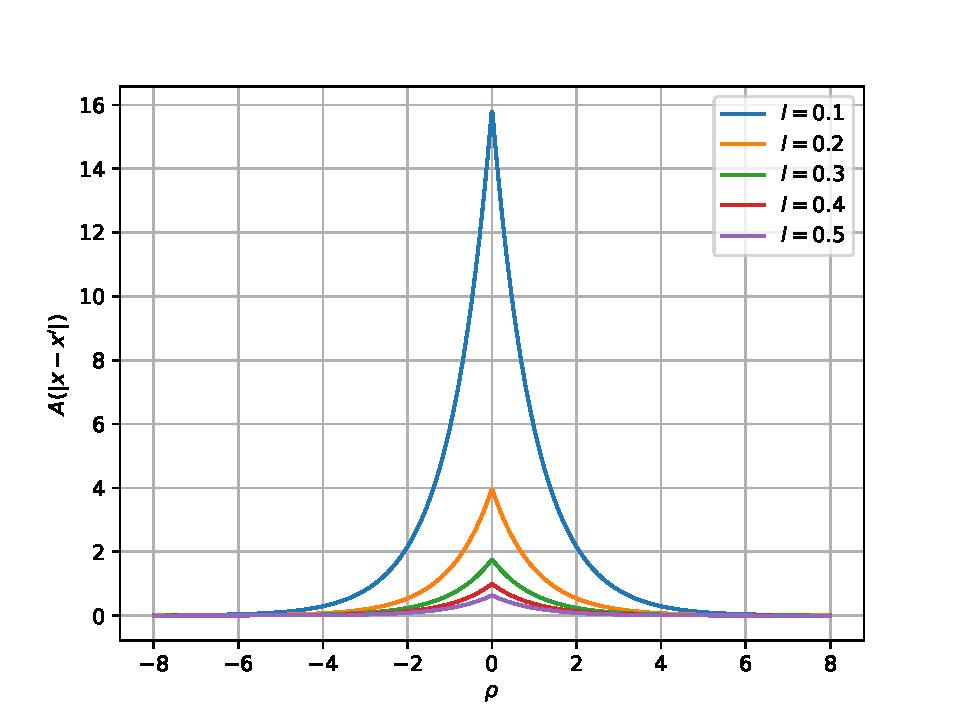
\includegraphics[width=\textwidth]{figuras/biexp2dl.pdf}
        \caption{Función 1}
        \label{fig:atenuacion_completa.f1}
    \end{subfigure}
    \begin{subfigure}{0.48\textwidth}
    \centering
        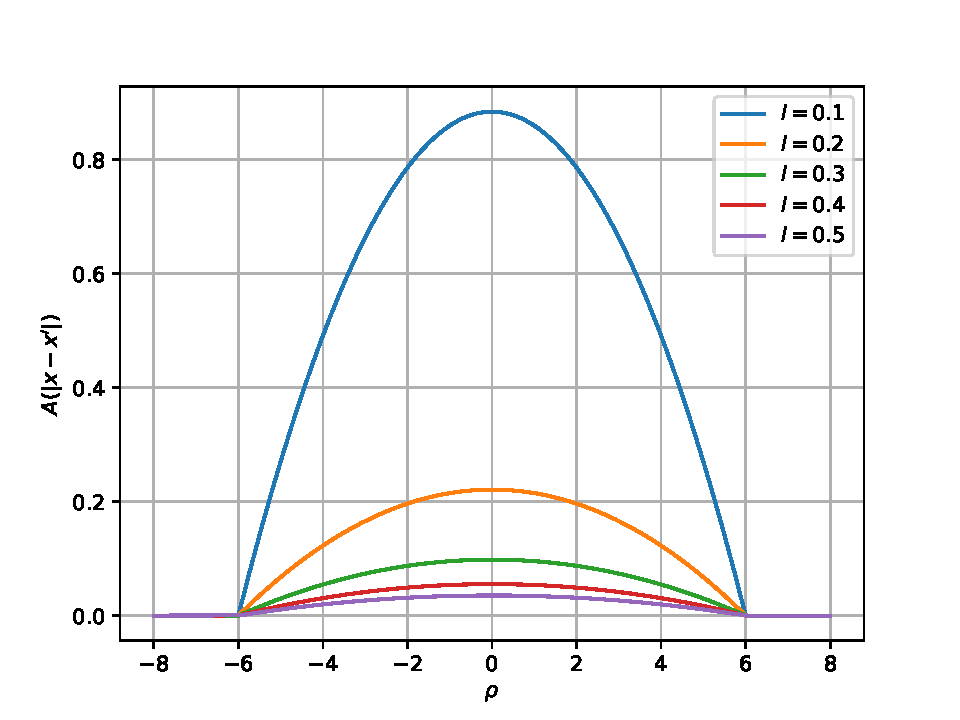
\includegraphics[width=\textwidth]{figuras/campana2dl.pdf}
        \caption{Función 2}
        \label{fig:atenuacion_completa.f2}
    \end{subfigure}
	\quad
    \begin{subfigure}{0.48\textwidth}
    \centering
        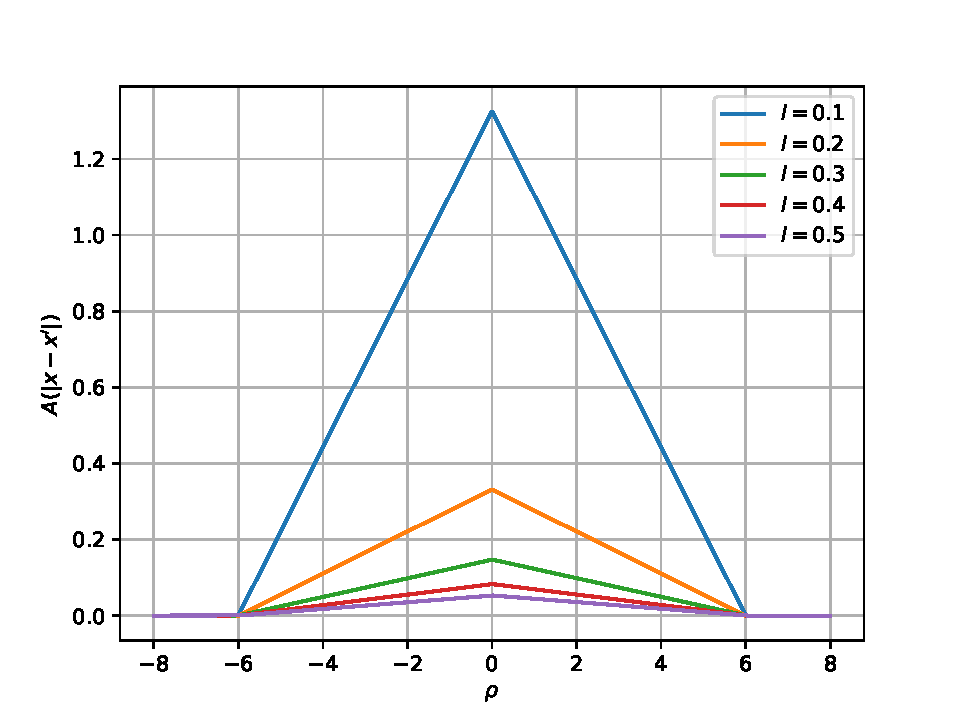
\includegraphics[width=\textwidth]{figuras/conica2dl.pdf}
        \caption{Función 3}
        \label{fig:atenuacion_completa.f3}
    \end{subfigure}
    \caption{Funciones de atenuación}
    \label{fig:atenuacion_completa}
\end{figure}	

\subsection{Función de Atenuación Modificada (Función 4)}

En el artículo \citetitle*{Pisano2009} se expone una metodología basada en el método de elementos finitos, el cual adopta el nombre de NL-FEM donde:

\begin{equation}
	\boldsymbol{\hat{K}U}=\boldsymbol{F}
\end{equation}
Donde $\boldsymbol{\hat{K}}$
\begin{equation}
	\boldsymbol{\hat{K}}=\sum_{n=1}^{N}{\left[\zeta_1\boldsymbol{K_n^{l}}+\zeta_2\sum_{m=1}^{M}\boldsymbol{K_{nm}^{nl}}\right]}
\end{equation}
Esto sugiere que para cada elemento $n$ existe un número $M$ de elementos no locales $m$ que se encuentran a una distancia de influencia $Lr$. Ademas, cuando $n=m$, $\boldsymbol{K^{nl}}$ se llama matriz de rigidez directa. Siguiendo la ecuación \ref{eq:eringen} es intuitivo pensar que la matriz de rigidez directa debe ser igual a la matriz de rigidez local, sin embargo, a nivel de elemento no se da esta igualdad, ya que en la integración numérica si existe una distancia entre los puntos de integración. Este efecto hace que:
\begin{equation}
	\zeta_1\boldsymbol{K_{n}^{l}}+\zeta_2\boldsymbol{K_{nn}^{nl}}\neq\boldsymbol{K_{n}^{l}}
\end{equation}
Por ello, se definió una función de atenuación la cual cumpla que $A(0)=0$ por lo que se optó por:
\begin{equation}
	A(\rho)=\lambda_0\rho e^{-\rho}
\end{equation}
Esta función tiene el comportamiento mostrado en la figura \ref{fig:modificada}.

\begin{figure}
    \centering
    \sffamily
    \begin{subfigure}{0.48\textwidth}
    \centering
        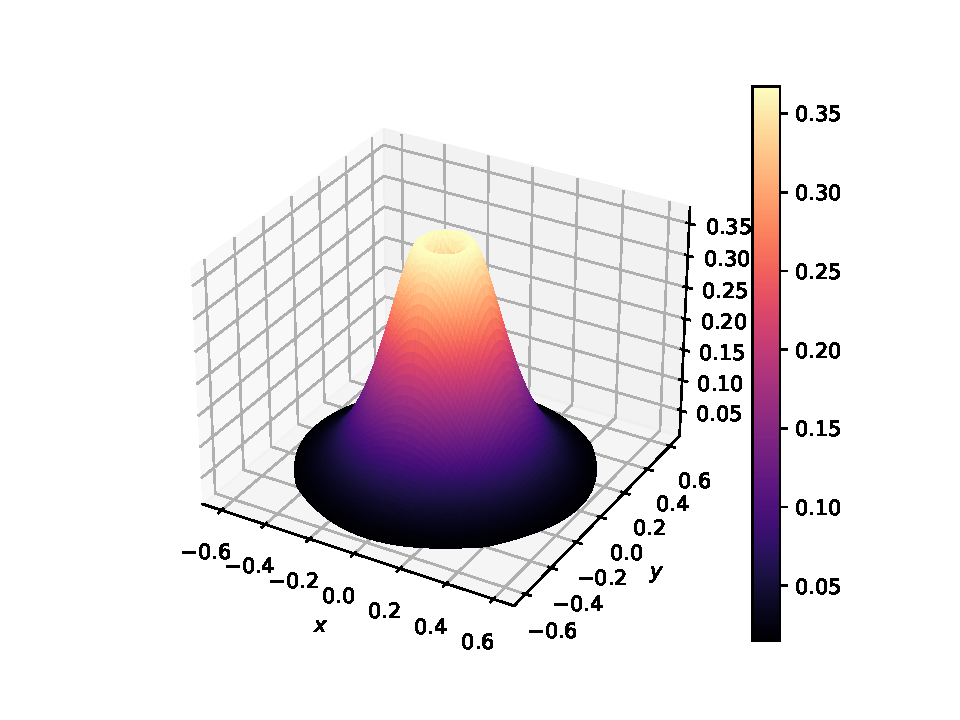
\includegraphics[width=\textwidth]{figuras/modificada3d.pdf}
        \caption{Superficie 3D}
        \label{fig:modificada.3d}
    \end{subfigure}
    \begin{subfigure}{0.48\textwidth}
    \centering
        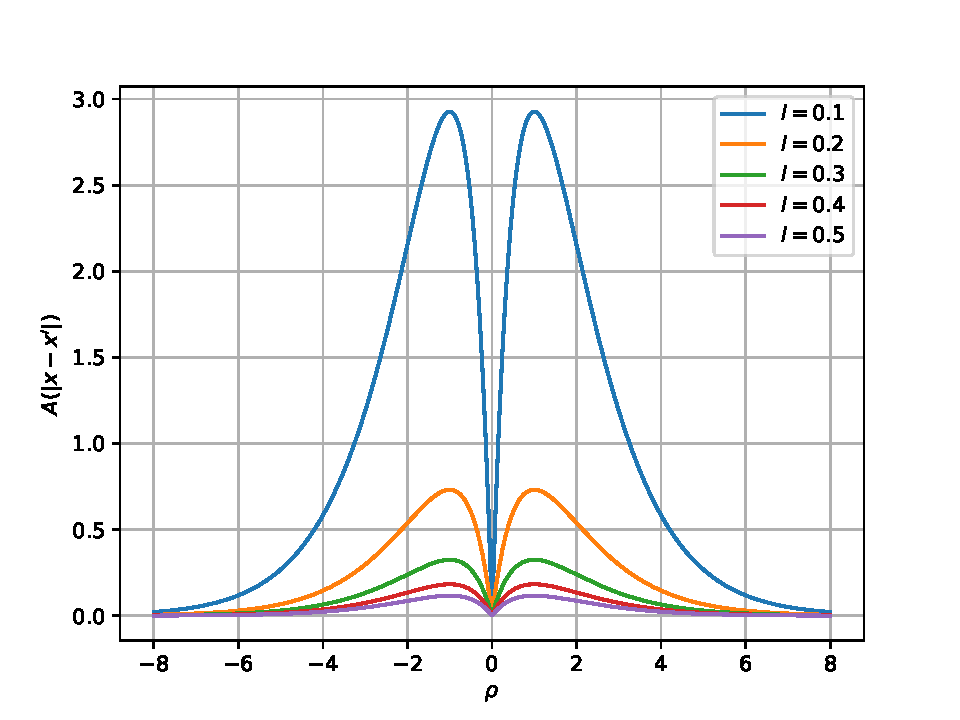
\includegraphics[width=\textwidth]{figuras/modificada2dl.pdf}
        \caption{Corte transversal}
        \label{fig:modificada.sublabel}
    \end{subfigure}
    \caption{Función de atenuación modificada}
    \label{fig:modificada}
\end{figure}

Adicionalmente se encontró que para que se cumpla la ecuación \ref{eq:condicion} se necesita:
\begin{equation}
	\lambda_0=\frac{1}{4\pi l^2}
\end{equation}
% \subsection{Página de mas alla, condiciones extra para quitarnos el \texorpdfstring{$\zeta_1$}{ζ1}}